% =====================================================================
% DGM (COMP 690-204) Final Project Proposal — camera-ready CVPR body content
% -----------------------------------------------------------------
% Paste into the official CVPR 2026 Overleaf template's \begin{document}:
%   https://www.overleaf.com/latex/templates/cvpr-2026-submission-template/rdtrwgypxxzb
% Use \usepackage{cvpr} (NOT \usepackage[review]{cvpr}) — this is a course
% proposal with your name on it, not an anonymous review submission.
% Upload outputs/figures/dgm/proposal_fig1.png to the Overleaf project
% before compiling (drag-and-drop into its file panel).
% =====================================================================

\title{Composition-Aware Cycle-Consistent Domain Translation \\ for Single-Cell and Bulk Transcriptomics}
\author{Arushi Sahai\thanks{COMP 690-204: Deep Generative Models --- Course Final Project Proposal.}}

\begin{document}
\maketitle

\setlength{\abovedisplayskip}{3pt}
\setlength{\belowdisplayskip}{3pt}
\setlength{\abovedisplayshortskip}{2pt}
\setlength{\belowdisplayshortskip}{2pt}
\setlength{\textfloatsep}{6pt plus 1pt minus 1pt}
\setlength{\abovecaptionskip}{3pt}
\setlength{\belowcaptionskip}{2pt}

\section{Overview}
Real biological datasets are rarely collected the same way every time. Different measurement batches, instruments,
or protocols introduce systematic variation mixed in with the biological signal of interest. In genomics,
this technical disparity is called a batch effect; resolving it means removing the non-biological variance
without losing the real signal underneath.

We focus on one clear, structured batch effect, studied here in a paired dataset of single-cell and
bulk RNA-seq from the same blood draws. RNA sequencing quantifies gene activity within a sample:
bulk RNA-seq averages expression across every cell in the sample, whereas single-cell RNA-seq (scRNA-seq)
profiles individual cells at higher resolution. In this cohort, single-cell RNA-seq is
performed on PBMC (peripheral blood mononuclear cells) while bulk RNA-seq uses whole blood --- different
preparations from the same draw, so despite identical donor biology, the profiles still look
different in a consistent way. This difference comes mainly from cell-type
composition: PBMC isolation physically depletes
granulocytes (50--70\% of whole blood), which bulk assays retain. CytoSet~\cite{yi2021cytoset}, a
permutation-invariant set encoder that pools single cells for sample-level prediction, is trained on
single-cell data in this cohort to classify donors as young or old. Its embedding space is organized by
assay identity instead of by age, so predictions do not transfer when the same encoder is applied to
bulk profiles. Standard batch-correction methods (ComBat, CORAL) pull the single-cell and bulk
embeddings closer together in that space (Figure~\ref{fig:proposal}). This correction distorts the
non-linear biological signal itself instead of removing only the technical difference, so
transfer does not recover. We frame this project as
domain-to-domain translation: learning a non-linear, cycle-consistent adversarial mapping (CyCADA-style).
The mapping is supervised by a task-consistency loss tied directly to real, measured immune-cell
composition.

\section{Related Work}
CycleGAN~\cite{zhu2017cyclegan} introduced cycle-consistency for unpaired image translation.
CyCADA~\cite{hoffman2018cycada} added task-consistency for domain adaptation, but targeted vision
classification with discrete cross-entropy objectives. We therefore replace
CyCADA's classification loss with a continuous regression loss, applied to 5000-dimensional gene
expression vectors instead of
images. Standard
genomics baselines
ComBat~\cite{johnson2007combat} and CORAL~\cite{sun2016coral} apply linear corrections that cannot model
asymmetric cell-type depletion; neither closes the gap in our evaluation (Figure~\ref{fig:proposal}).
Recent transcriptomic
GANs apply to different settings: GANomics~\cite{wu2026ganomics} bridges microarray and RNA-seq platforms on
identical tissue extracts rather than distinct cell preparations from the same draw.
STCGAN~\cite{wang2025stcgan} pretrains a cycle-consistent GAN, then estimates composition afterward
in a separate module, two decoupled stages. Our approach differs: composition is the task-consistency
signal inside the generator's own training loop from the start, one objective, not two.

\section{Approach}
Both domains are represented as 5000-dimensional vectors, log-normalized to a common total count per
sample (log-CP10k, a standard RNA-seq scaling), over a shared gene panel (the genes reliably detected by
both assays), so each dimension refers to the same gene in both domains.
Single-cell data is aggregated into sample-level pseudobulk, $x_S \in \mathcal{S}$, by summing counts per
sample so the result resembles a real bulk profile. Bulk data is represented as $x_B \in \mathcal{B}$.
Operating on pseudobulk rather than individual cells preserves a fixed-dimensional metric space, needed
for discriminator stability and tractable $\ell_1$ cycle-consistency. Modeling raw single cells would
instead require set-level discriminators and set-to-set distances (e.g., optimal transport), which are
notoriously difficult to train reliably; bulk profiles also lack cell-level
resolution to target directly. Pseudobulk is also the representation on which cross-domain signal survives, a main result from our
ongoing CytoSet benchmarking study. The set encoder configuration (Overview) induces collapse instead.

Generators $G_{S \to B}$ and $G_{B \to S}$ are parameterized as residual MLPs
($G(x) = x + \text{MLP}(x)$, $5000 \to 512 \to 512 \to 5000$). The residual principle is established,
echoing how CycleGAN's own generators avoid reconstructing from scratch. Applying it as a flat MLP over
tabular gene-expression vectors, rather than CycleGAN's convolutional image architecture, is our own
design choice. ComBat and CORAL are both linear corrections, so neither can capture non-linear structure in the shift
between domains; the learned MLP adds that non-linear correction on top. Keeping the correction
additive, instead of generating the output from scratch, keeps the generator anchored to the real input
and unable to destroy real biological signal while correcting it.

Discriminators $D_S$ and $D_B$ are MLPs trained with the established LSGAN objective~\cite{mao2017lsgan}.
The $S \to B$ direction is optimized as
$\min_{G_{S \to B}} \max_{D_B}$:
\begin{equation}
\mathcal{L}_{\text{adv}}^{S \to B} = \mathbb{E}_{x_B}[(D_B(x_B){-}1)^2] + \mathbb{E}_{x_S}[D_B(G_{S \to B}(x_S))^2],
\end{equation}
A symmetric $\mathcal{L}_{\text{adv}}^{B \to S}$ covers the reverse direction, and the total adversarial term used below is
$\mathcal{L}_{\text{adv}} = \mathcal{L}_{\text{adv}}^{S \to B} + \mathcal{L}_{\text{adv}}^{B \to S}$.
Cycle-consistency follows CycleGAN~\cite{zhu2017cyclegan} directly:
\begin{equation}
\begin{split}
\mathcal{L}_{\text{cyc}} = &\ \mathbb{E}_{x_S}[\|G_{B \to S}(G_{S \to B}(x_S)) - x_S\|_1] \\
&+ \mathbb{E}_{x_B}[\|G_{S \to B}(G_{B \to S}(x_B)) - x_B\|_1].
\end{split}
\end{equation}
Both of the above are established machinery, unchanged from prior work.

This is where our approach departs from CyCADA. Instead of a classifier trained on a proxy label, the
task loss uses two regressors, $C_{\text{bulk}}$ and $C_{\text{sc}}$, which predict cell-type
composition (the fraction of a sample's cells in each major immune lineage, such as T cells, B cells, or
monocytes) as a vector on the simplex $\Delta^{K-1}$, computed directly from established single-cell
annotations.
Matched pairs originate from the same draw, so one invariant ground-truth composition vector, $c^*$,
supervises both directions without deconvolution. $c^*$ is measured directly from real biology, not
predicted by a model. This is the point where biology drives the objective directly.
Both task networks are pretrained to convergence and frozen. Our mathematical contribution is this
task-consistency term:
\begin{equation}
\mathcal{L}_{\text{task}} = \|C_{\text{bulk}}(G_{S \to B}(x_S)) - c^*\|_1 +
\|C_{\text{sc}}(G_{B \to S}(x_B)) - c^*\|_1.
\end{equation}
The full objective follows CyCADA's~\cite{hoffman2018cycada} structure, with this term substituted for
its classification-based one: $\mathcal{L} = \mathcal{L}_{\text{adv}} + \lambda_{\text{cyc}}
\mathcal{L}_{\text{cyc}} + \lambda_{\text{task}} \mathcal{L}_{\text{task}}$.

\section{Experiments}
\textbf{Data:} We evaluate on AIFI Sound Life~\cite{gustafson2025soundlife}: 96 healthy donors, each with a matched single-cell (on
PBMC) and bulk (on whole-blood) sample pair from the same draw, for $\sim$840 pairs total (public, CC BY
4.0). This same-draw matching ensures the domain gap reflects measurement assay
differences, not donor identity or draw timing. Splits are donor-grouped, since donors contribute
multiple samples; preprocessing and loaders are pre-constructed. At $\sim$840 pairs, this is a modest sample size for GAN training --- a real limitation
on what the evaluation below can establish.

\textbf{Baselines \& Evaluation:} We benchmark against uncorrected data, ComBat, and CORAL, and report:
\textbf{(1) Domain Alignment} --- reductions in the silhouette score (how separated the two domains are
in the embedding, where lower is better) and in how much of the top principal component reflects
modality, not biology; \textbf{(2) Downstream Transfer} --- evaluating corrected profiles on CytoSet's
original task, with its weights frozen, classifying donors as young or old, scored by AUROC;
\textbf{(3) Translation Accuracy} ---
per-sample correlation ($R^2$, Spearman $\rho$) with the real paired profile, plus per-gene mean/variance
agreement; \textbf{(4) Task Generalization} --- composition-prediction accuracy on donors held out from
both task-net pretraining and GAN training, testing whether the signal generalizes rather than being
memorized; and \textbf{(5) Sanity Checks} --- per-sample output diversity, held-out cycle-reconstruction
error, and whether marker genes (e.g., CD3D/CD3E for T cells) still show the expected pattern after
translation.

\textbf{Ablations:} Each ablation tests a specific design decision from Approach rather than sweeping an
arbitrary hyperparameter, ordered from most fundamental to most specific: \textbf{(1) No Task Loss} ---
training with only the adversarial and cycle-consistency terms ($\lambda_{\text{task}} = 0$), the plain
CycleGAN case, to establish whether task-consistency contributes anything beyond cycle-consistency alone;
\textbf{(2) Task Loss Type} --- swapping $C_{\text{bulk}}$/$C_{\text{sc}}$ for CytoSet's frozen
young-vs-old classifier, CyCADA's original classification-based formulation, to test whether real
biology grounds the task loss better than a generic signal; and
\textbf{(3) Generator Architecture} --- comparing the residual generator ($G(x) = x + \text{MLP}(x)$)
against a non-residual MLP of the same capacity, to test whether the additive property is actually what
protects biological signal during translation, as Approach claims.

\section{Others}
We want to know two things: whether our translation approach can close the single-cell/bulk preparation
gap without erasing the signal that matters for prediction, and whether grounding the task loss in real
biology works better than a generic classifier would.

Uncertainties remain: GAN training is known to be unstable in general, and whether that holds at this
sample size and dimensionality ($\sim$840 pairs, 5000 dimensions) is untested. PBMCs completely lack
granulocytes, requiring $G_{S \to B}$ to reconstruct granulocyte-associated gene expression from how
other genes co-vary alone. This approach also relies on same-draw pairing for ground-truth composition,
unavailable in our broader study's unmatched cohorts.

\begin{figure}[t]
  \centering
  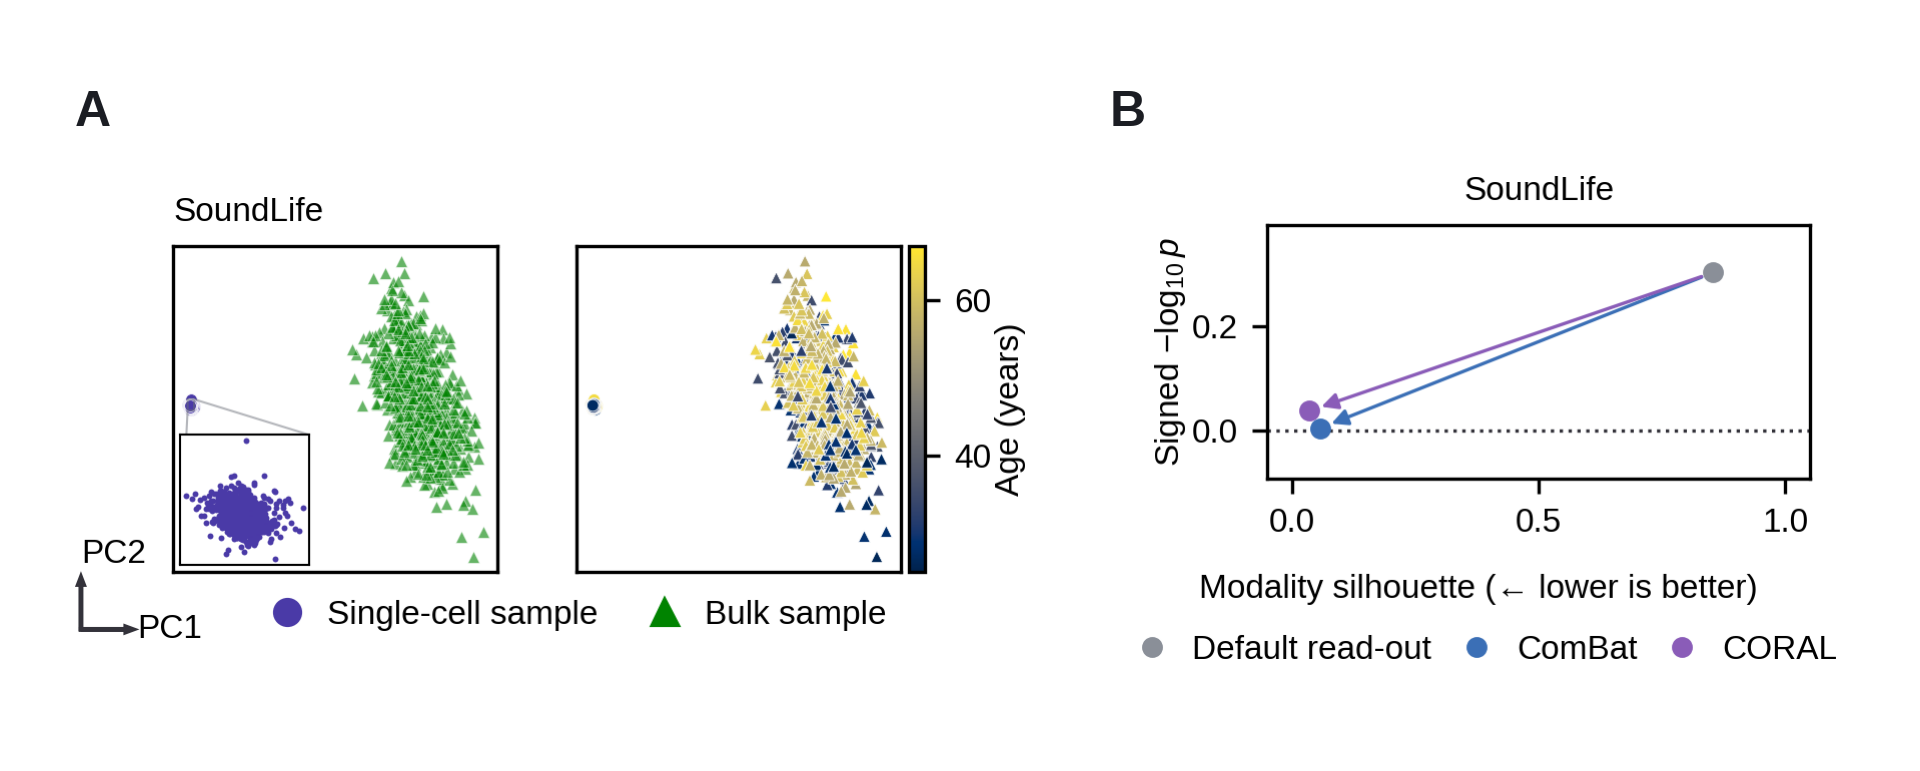
\includegraphics[width=\linewidth, height=0.30\textheight, keepaspectratio]{proposal_fig1.png}
  \caption{(a) Joint PCA of CytoSet's embedding for single-cell and bulk samples (AIFI Sound Life), colored by
  modality (single-cell samples enlarged in an inset) and by age. PC1 separates the assays, not age
  (silhouette 0.85, PC1 $\eta^2$ modality 0.98, age $<0.01$). (b) Modality silhouette of the embeddings in
  (a) against young-vs-old transfer (signed $-\log_{10} p$) for the default read-out (gray; its LASSO
  z-scores each assay on its own) and after ComBat or CORAL: both corrections collapse the silhouette
  from 0.85 to 0.06 and 0.04 without recovering transfer, which stays at chance.}
  \label{fig:proposal}
\end{figure}

\end{document}

% -----------------------------------------------------------------
% .bib entries needed (author/venue/year verified against primary sources
% earlier this session):
%   zhu2017cyclegan     Zhu, Park, Isola, Efros. Unpaired Image-to-Image
%                       Translation using Cycle-Consistent Adversarial
%                       Networks. ICCV 2017.
%   hoffman2018cycada   Hoffman, Tzeng, Park, Zhu, Isola, Saenko, Efros,
%                       Darrell. CyCADA: Cycle-Consistent Adversarial
%                       Domain Adaptation. ICML 2018.
%   johnson2007combat   Johnson, Li, Rabinovic. Adjusting batch effects in
%                       microarray expression data using empirical Bayes
%                       methods. Biostatistics 8(1):118-127, 2007.
%   sun2016coral        Sun, Feng, Saenko. Return of Frustratingly Easy
%                       Domain Adaptation. AAAI 2016. (NOT "Deep CORAL" —
%                       see the earlier verification note; this repo's
%                       coral_correct_domains is the original 2016 method.)
%   wu2026ganomics      Wu, Salman, Tong. GANomics: bridging legacy and
%                       modern transcriptomic platforms for clinical
%                       applications. npj Genomic Medicine, 2026.
%   wang2025stcgan      Wang, Long, Bai, Luo, Kwoh. STCGAN: a novel
%                       cycle-consistent generative adversarial network
%                       for spatial transcriptomics cellular
%                       deconvolution. Briefings in Bioinformatics
%                       26(1):bbae670, 2025.
%   yi2021cytoset      Yi, Stanley. CytoSet: Predicting clinical outcomes
%                       via set-modeling of cytometry data. ACM-BCB 2021.
%   mao2017lsgan        Mao, X.; Li, Q.; Xie, H.; Lau, R.Y.K.; Wang, Z.;
%                       Smolley, S.P. Least Squares Generative Adversarial
%                       Networks. ICCV 2017, pp. 2813-2821.
%                       DOI 10.1109/ICCV.2017.304 (verified 2026-09-30).
%                       Cited inline in Approach only, at the LSGAN
%                       equation -- not in Related Work, since it's an
%                       implementation-level loss choice, not a competing
%                       or foundational approach to the problem itself.
%   gustafson2025soundlife  Gustafson, C.E., et al. Multi-omic profiling
%                       reveals age-related immune dynamics in healthy
%                       adults. Nature 648:696-706 (2025).
%                       DOI 10.1038/s41586-025-09686-5. Verified
%                       2026-09-30 -- this is the peer-reviewed publication
%                       of the preprint formerly at bioRxiv
%                       10.1101/2024.09.10.612119 (superseded, do not cite
%                       that one). Lead author is Gustafson, not "Gong" as
%                       an earlier note had it.
% -----------------------------------------------------------------
